\documentclass{article}
\usepackage{amsmath,amssymb,amsthm}
\usepackage{enumerate,mathtools}
\usepackage{tikz}
\usepackage{hyperref}
\usepackage{algorithm2e}
\usepackage[letterpaper,margin=1in]{geometry}

\makeatletter
\let\Hy@linktoc\Hy@linktoc@none
\makeatother

% Theorems
\usepackage{amsthm}
\renewcommand\qedsymbol{$\blacksquare$}

\newtheorem{definition}{Definition}[section]
\newtheorem{example}{Example}[section]
\newtheorem{theorem}{Theorem}[section]
\newtheorem{corollary}[theorem]{Corollary}
\newtheorem{lemma}[theorem]{Lemma}


% Linear Algebra %

\setlength\unitlength{1mm}

\newcommand{\insertfig}[3]{
\begin{figure}[htbp]\begin{center}\begin{picture}(120,90)
\put(0,-5){\includegraphics[width=12cm,height=9cm,clip=]{#1.eps}}\end{picture}\end{center}
\caption{#2}\label{#3}\end{figure}}

\newcommand{\insertxfig}[4]{
\begin{figure}[htbp]
\begin{center}
\leavevmode \centerline{\resizebox{#4\textwidth}{!}{\input
#1.pstex_t}}
%\vspace*{-0.2in}
\caption{#2} \label{#3}
\end{center}
\end{figure}}

\long\def\comment#1{}

\newcommand\norm[1]{\left\lVert#1\right\rVert}
\DeclareMathOperator*{\argmin}{arg\,min}
\DeclareMathOperator*{\argmax}{arg\,max}
% bb font symbols

\newfont{\bbb}{msbm10 scaled 700}
\newcommand{\CCC}{\mbox{\bbb C}}

\newfont{\bbf}{msbm10 scaled 1100}
\newcommand{\CC}{\mbox{\bbf C}}
\newcommand{\PP}{\mbox{\bbf P}}
\newcommand{\RR}{\mbox{\bbf R}}
\newcommand{\QQ}{\mbox{\bbf Q}}
\newcommand{\ZZ}{\mbox{\bbf Z}}
\renewcommand{\SS}{\mbox{\bbf S}}
\newcommand{\FF}{\mbox{\bbf F}}
\newcommand{\GG}{\mbox{\bbf G}}
\newcommand{\EE}{\mbox{\bbf E}}
\newcommand{\NN}{\mbox{\bbf N}}
\newcommand{\KK}{\mbox{\bbf K}}

% Vectors

\renewcommand{\aa}{{\bf a}}
\newcommand{\bb}{{\bf b}}
\newcommand{\cc}{{\bf c}}
\newcommand{\dd}{{\bf d}}
\newcommand{\ee}{{\bf e}}
\newcommand{\ff}{{\bf f}}
\renewcommand{\gg}{{\bf g}}
\newcommand{\hh}{{\bf h}}
\newcommand{\ii}{{\bf i}}
\newcommand{\jj}{{\bf j}}
\newcommand{\kk}{{\bf k}}
\renewcommand{\ll}{{\bf l}}
\newcommand{\mm}{{\bf m}}
\newcommand{\nn}{{\bf n}}
\newcommand{\oo}{{\bf o}}
\newcommand{\pp}{{\bf p}}
\newcommand{\qq}{{\bf q}}
\newcommand{\rr}{{\bf r}}
\renewcommand{\ss}{{\bf s}}
\renewcommand{\tt}{{\bf t}}
\newcommand{\uu}{{\bf u}}
\newcommand{\ww}{{\bf w}}
\newcommand{\vv}{{\bf v}}
\newcommand{\xx}{{\bf x}}
\newcommand{\yy}{{\bf y}}
\newcommand{\zz}{{\bf z}}
\newcommand{\0}{{\bf 0}}
\newcommand{\1}{{\bf 1}}

% Matrices

\newcommand{\Ab}{{\bf A}}
\newcommand{\Bb}{{\bf B}}
\newcommand{\Cb}{{\bf C}}
\newcommand{\Db}{{\bf D}}
\newcommand{\Eb}{{\bf E}}
\newcommand{\Fb}{{\bf F}}
\newcommand{\Gb}{{\bf G}}
\newcommand{\Hb}{{\bf H}}
\newcommand{\Ib}{{\bf I}}
\newcommand{\Jb}{{\bf J}}
\newcommand{\Kb}{{\bf K}}
\newcommand{\Lb}{{\bf L}}
\newcommand{\Mb}{{\bf M}}
\newcommand{\Nb}{{\bf N}}
\newcommand{\Ob}{{\bf O}}
\newcommand{\Pb}{{\bf P}}
\newcommand{\Qb}{{\bf Q}}
\newcommand{\Rb}{{\bf R}}
\newcommand{\Sb}{{\bf S}}
\newcommand{\Tb}{{\bf T}}
\newcommand{\Ub}{{\bf U}}
\newcommand{\Wb}{{\bf W}}
\newcommand{\Vb}{{\bf V}}
\newcommand{\Xb}{{\bf X}}
\newcommand{\Yb}{{\bf Y}}
\newcommand{\Zb}{{\bf Z}}

% Calligraphic

\newcommand{\Ac}{{\cal A}}
\newcommand{\Bc}{{\cal B}}
\newcommand{\Cc}{{\cal C}}
\newcommand{\Dc}{{\cal D}}
\newcommand{\Ec}{{\cal E}}
\newcommand{\Fc}{{\cal F}}
\newcommand{\Gc}{{\cal G}}
\newcommand{\Hc}{{\cal H}}
\newcommand{\Ic}{{\cal I}}
\newcommand{\Jc}{{\cal J}}
\newcommand{\Kc}{{\cal K}}
\newcommand{\Lc}{{\cal L}}
\newcommand{\Mc}{{\cal M}}
\newcommand{\Nc}{{\cal N}}
\newcommand{\Oc}{{\cal O}}
\newcommand{\Pc}{{\cal P}}
\newcommand{\Qc}{{\cal Q}}
\newcommand{\Rc}{{\cal R}}
\newcommand{\Sc}{{\cal S}}
\newcommand{\Tc}{{\cal T}}
\newcommand{\Uc}{{\cal U}}
\newcommand{\Wc}{{\cal W}}
\newcommand{\Vc}{{\cal V}}
\newcommand{\Xc}{{\cal X}}
\newcommand{\Yc}{{\cal Y}}
\newcommand{\Zc}{{\cal Z}}

% Bold greek letters

\newcommand{\alphab}{\hbox{\boldmath$\alpha$}}
\newcommand{\betab}{\hbox{\boldmath$\beta$}}
\newcommand{\gammab}{\hbox{\boldmath$\gamma$}}
\newcommand{\deltab}{\hbox{\boldmath$\delta$}}
\newcommand{\etab}{\hbox{\boldmath$\eta$}}
\newcommand{\lambdab}{\hbox{\boldmath$\lambda$}}
\newcommand{\epsilonb}{\hbox{\boldmath$\epsilon$}}
\newcommand{\nub}{\hbox{\boldmath$\nu$}}
\newcommand{\mub}{\hbox{\boldmath$\mu$}}
\newcommand{\zetab}{\hbox{\boldmath$\zeta$}}
\newcommand{\phib}{\hbox{\boldmath$\phi$}}
\newcommand{\psib}{\hbox{\boldmath$\psi$}}
\newcommand{\thetab}{\hbox{\boldmath$\theta$}}
\newcommand{\taub}{\hbox{\boldmath$\tau$}}
\newcommand{\omegab}{\hbox{\boldmath$\omega$}}
\newcommand{\xib}{\hbox{\boldmath$\xi$}}
\newcommand{\sigmab}{\hbox{\boldmath$\sigma$}}
\newcommand{\pib}{\hbox{\boldmath$\pi$}}
\newcommand{\rhob}{\hbox{\boldmath$\rho$}}

\newcommand{\Gammab}{\hbox{\boldmath$\Gamma$}}
\newcommand{\Lambdab}{\hbox{\boldmath$\Lambda$}}
\newcommand{\Deltab}{\hbox{\boldmath$\Delta$}}
\newcommand{\Sigmab}{\hbox{\boldmath$\Sigma$}}
\newcommand{\Phib}{\hbox{\boldmath$\Phi$}}
\newcommand{\Pib}{\hbox{\boldmath$\Pi$}}
\newcommand{\Psib}{\hbox{\boldmath$\Psi$}}
\newcommand{\Thetab}{\hbox{\boldmath$\Theta$}}
\newcommand{\Omegab}{\hbox{\boldmath$\Omega$}}
\newcommand{\Xib}{\hbox{\boldmath$\Xi$}}


% mixed symbols

\newcommand{\sinc}{{\hbox{sinc}}}
\newcommand{\diag}{{\hbox{diag}}}
\renewcommand{\det}{{\hbox{det}}}
\newcommand{\trace}{{\hbox{tr}}}
\newcommand{\tr}{\trace}
\newcommand{\sign}{{\hbox{sign}}}
\renewcommand{\arg}{{\hbox{arg}}}
\newcommand{\var}{{\hbox{var}}}
\newcommand{\cov}{{\hbox{cov}}}
\renewcommand{\Re}{{\rm Re}}
\renewcommand{\Im}{{\rm Im}}
\newcommand{\eqdef}{\stackrel{\Delta}{=}}
\newcommand{\defines}{{\,\,\stackrel{\scriptscriptstyle \bigtriangleup}{=}\,\,}}
\newcommand{\<}{\left\langle}
\renewcommand{\>}{\right\rangle}
\newcommand{\Psf}{{\sf P}}
\newcommand{\T}{\top}
\newcommand{\m}[1]{\begin{bmatrix} #1 \end{bmatrix}}


\setlength{\parindent}{0pt}

\begin{document}

\begin{center}
  \Large\textbf{Convex Optimization Overview}\\
  \large\textit{Conner DiPaolo}
\end{center}
\vspace*{1em}

\tableofcontents
\vspace{1em}

\section{Introduction}

Convex optimization in a large way influences the way
people think about and phrase machine learning problems.
Almost all problems we will see in our studies are developed
or can be viewed as optimization problems. Some problems,
like the Support Vector Machine you will all see in the coming
weeks, are almost entirely based in the heart of convex optimization.\\

We don't plan on bringing you all up to speed completely on
the art of Convex Optimization, but hopefully in two sections you
will know enough to be able to think about problems in new, interesting
ways that will aid your studies in and out of machine learning.\\

The only real prerequisite for this material is a strong confidence
in linear algebra and familiarity with matrix calculus. Note that
much of this material stems from Boyd and Vandenberghe's insanely influential
textbook \textit{Convex Optimization}. If you are interested in the
topic or need a more in-depth resource, check out the book. It's free
online\footnote{\url{http://stanford.edu/~boyd/cvxbook/}}.

%%%%%%%%%%%%%%%%%%%%%%%%%%%%%%%%%%%%%%%%%%%%
\section{Convex Sets}



The first step into examining convexity is defining what a
\textbf{convex set} is when given, for example, a subset of the real numbers,
or the set of matrices.

\begin{figure}
    \centering
    \begin{center}
        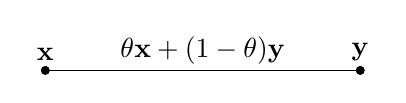
\begin{tikzpicture}
            \draw[fill=black] (0,0) circle (0.05) node[above] {$\xx$};
            \draw[fill=black] (4,0) circle (0.05) node[above] {$\yy$};
            \draw (0,0) -- (4,0);
            \draw (2,0.25) node {$\theta\xx + (1-\theta)\yy$};
        \end{tikzpicture}
    \end{center}
    \caption{\textbf{Convex Combination}. The line segment between $\xx$ and $\yy$ 
    above represents every possible combination $\{\theta\xx + (1-\theta)\yy : 
    0\leq\theta\leq1\}$.}
    \label{fig:convex-comb}
\end{figure}

\begin{definition}[Convex Combination]
    In the $n=2$ case, the convex combination of points $\xx$ and $\yy$ in an
    affine space is
    \[
        \theta\xx + (1-\theta)\yy
    \]
    where $0\leq\theta\leq1$. Intuitively, this is the line segment between
    $\xx$ and $\yy$ (consider $\theta=0$ and $\theta=1$), as seen in Figure
    \ref{fig:convex-comb}. More generally,
    a convex combination of points $\xx_1,\xx_2,\dots,\xx_n$ in an affine space (vector
    spaces included) is the combination
    \[
        \thetab_1\xx_1 + \thetab_2\xx_2 + \dots + \thetab_n\xx_n = \thetab^\T\xx
    \]
    where $\theta_i \geq 0$ and $\1^\T\theta = 1$. That is, $\thetab$ lies on the
    standard probability simplex.  
\end{definition}

With this definition of a convex combination we can define
a convex set:

\begin{figure}
    \centering
    \begin{center}
        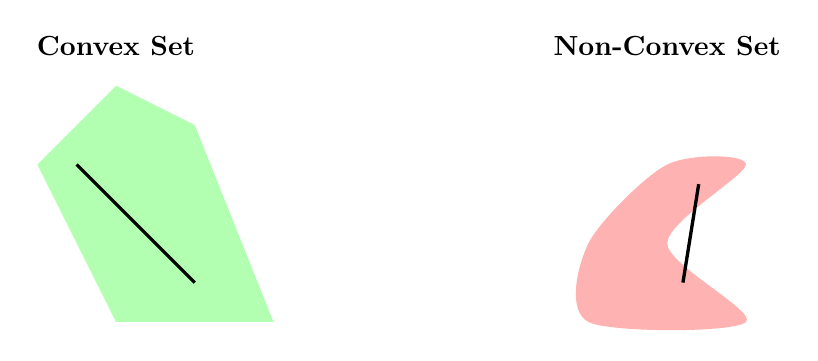
\begin{tikzpicture}
            \begin{scope}[shift={(-3,0)}]
                \draw (0,3.5) node {\textbf{Convex Set}};
                \fill[color=green!30] (0,0) -- (-1,2) -- (0,3) -- (1,2.5) -- (2,0)  -- cycle;
                \draw[very thick] (-0.5,2) -- (1,0.5);
            \end{scope}
            \begin{scope}[shift={(3,0)}]
                \draw (1,3.5) node {\textbf{Non-Convex Set}};
                \fill[color=red!30] plot [smooth cycle] coordinates {(0,1) (1,2) (2,2) (1,1) (2,0) (0,0)};
                \draw[very thick] (1.4,1.75) -- (1.2,0.5);
            \end{scope}
        \end{tikzpicture}
    \end{center}
    \caption{{\bf Set convexity.} Intuitively, a set is convex
    if a line drawn between any two points within the set lies completely in the set. The convex set
    to the left is a \textit{convex hull} of it's vertices, meaning the set is constructed
    as all possible convex combinations of its vertices. These sets are subsets of $\RR^2$.}
    \label{fig:convex-sets}
\end{figure}

\begin{definition}[Convex Set]
    A set $C$ is convex if, given $\xx,\yy \in C$, every convex combination
    of $\xx$ and $\yy$ is still in $C$. Mathematically,
    \[
        \theta\xx + (1-\theta)\yy \in C. \tag{$0\leq\theta\leq1$}
    \]
    See Figure \ref{fig:convex-sets} for an illustration. Intuitively, this
    means that every line segment between any two points in $C$ is contained
    entirely within $C$.
\end{definition}

\subsection{Examples of Convex and Non-Convex Sets}

\begin{example}[All of $\RR^n$]
    $\RR^n$ is convex.
\end{example}
\begin{proof}
    As a vector space, for any $\theta_1,\theta_2 \in \RR$ and $\xx$ and
    $\yy$ in $\RR^n$,
    \[
        \theta_1 \xx + \theta_2 \yy \in \RR^n.
    \]
    Thus, restricting $\theta_2 = 1-\theta_1$ and $0\leq\theta_1\leq1$
    does not change this fact, and any convex combination is also in
    $\RR^n$, making the set convex by definition.
\end{proof}

\begin{example}[The Non-Negative Orthant $\RR^n_+$]
    The set of all vectors
    \[
        \{\xx : \xx\in\RR^n \text{ and } \xx_i \geq 0\}
    \]
    is convex.
\end{example}
\begin{proof}
    Left as an exercise to the reader.
\end{proof}

\begin{example}[Closed Intervals in $\RR$]
    \label{ex:closed-intervals-convex}
    Let $C = [a,b]$ be a subset of the real numbers where $a \leq b$.
    Then $C$ is convex.
\end{example}
\begin{proof}
    Suppose, without loss of generality, that $x_1 \leq x_2$ where
    $x_1,x_2 \in [a,b]$. Now let $0\leq\theta\leq1$. Then
    \[
        \theta x_1 + (1-\theta) x_2 \leq \theta x_2 + (1-\theta) x_2 = x_2
    \]
    because $\theta x_1 \leq \theta x_2$. Similarly,
    \[
        \theta x_1 + (1-\theta) x_2 \geq \theta x_1 + (1-\theta) x_1 = x_1
    \]
    because $(1-\theta) x_2 \geq (1-\theta) x_1$. Thus
    \[
        a \leq x_1 \leq \theta x_1 + (1-\theta) x_2 \leq x_2 \leq b,
    \]
    and hence
    \[
        \theta x_1 + (1-\theta) x_2 \in [a,b].
    \]
    Therefore, by the definition of convexity, $[a,b]\subseteq\RR$ is convex
    for any $a \leq b$.
\end{proof}

\begin{example}[The Set of All Complex Hermetian Matrices]
    \label{ex:hermitian-convex}
    Let $C = \{A : A\in\CC^{n\times n} \text{ and } A^* = A\}$. $C$ is
    convex.
\end{example}
\begin{proof}
    Let $A,B\in\CC^{n\times n}$ be Hermitian matrices and $0\leq\theta\leq1$.
    Then
    \begin{align}
        (\theta A + (1-\theta) B)^* &= (\theta A)^* + \left[(1-\theta)B\right]^*\\
        &= \theta A^* + (1-\theta) B^*\\
        &= \theta A + (1-\theta) B \tag{because $A^*=A$ and $B^*=B$}\\
    \end{align}
    Thus every convex combination of Hermitian matrices is Hermitian,
    and by the definition of convexity the set is convex.
\end{proof}

\begin{example}[The Set of All Real Symmetric Matrices]
    Let $C = \{A : A\in\RR^{n\times n} \text{ and } A^\T = A\}$. $C$ is
    convex.
\end{example}
\begin{proof}
    Left as an exercise to the reader.
\end{proof}

\begin{example}[The Set of All Linear Matrix Inequalities]
    Let $A_i$ and $B$ be symmetric $n\times n$ matrices and
    $\xx\in\RR^n$.
    Let $C = \{\xx : A(\xx) \preceq B\}$ where $A(\xx) = \xx_1A_1 +
    \dots + \xx_kA_k$. $C$ is convex.
\end{example}
\begin{proof}
    Let $0\leq\theta\leq1$ and $\xx, \yy \in C$. Then
    \begin{align*}
        A(\theta\xx + (1-\theta)\yy) &= \sum_i \left[ \theta\xx_i + (1-\theta)\yy_i \right]A_i\\
        &= \theta\sum_i \xx_i A_i + (1-\theta)\sum_i \xx_i A_i\\
        &= \theta A(\xx) + (1-\theta) A(\yy)\\
        &\leq \theta B + (1-\theta) B\\
        &= B.
    \end{align*}
    Thus any convex combination of elements of $C$ is contained
    in $C$ and by definition $C$ is convex.
\end{proof}

\begin{example}[The Space of Probability Distributions]
    Let $\Pc$ be the space of continuous probability distributions over
    $\RR^n$. That is, every element of $\Pc$ defines a unique probability
    density function $\PP(x) \geq 0$ such that \[\int_{\RR^n} \PP(x) dx=1.\]
    $\Pc$ is convex.
\end{example}
\begin{proof}
    Let $f$ and $h$ be valid probability distributions from $\Pc$. That is,
    \[
        f,h \in \left\{\PP(x) : \int_{\RR^n} \PP(x)dx = 1 \text{ and } \PP(x) \geq 0 \right\}.
    \]
    Now let $0\leq\theta\leq1$. Then
    \[
        \theta f(x) + (1-\theta) h(x) \geq 0
    \]
    as a positive combination of positive functions. Similarly,
    \begin{align*}
        \int_{\RR^n}\left[ \theta f(x) + (1-\theta) h(x) \right]dx &= \theta\int_{\RR^n}f(x)dx + (1-\theta)\int_{\RR^n}h(x)dx\\
        &= \theta + (1-\theta) = 1.
    \end{align*}
    Thus every convex combination of probability distributions over $\RR^n$ is
    a valid distribution (often called a mixture), and therefore the set of
    all valid probability distributions over $\RR^n$ is convex itself.
\end{proof}

\begin{example}[Disjoint Intervals in $\RR$]
    Let $N = [a,b] \cup [c,d]$ where $a\leq b < c \leq d$.
    $N$ is \textbf{not} convex.
\end{example}
\begin{proof}
    Let $b,c\in N$ be as described above. Then for $0<\theta<1$
    (not we aren't including inequality),
    \[
        \theta b + (1-\theta)c \not\in N.
    \]
    Thus not \textit{every} convex combination of elements in
    $N$ is in $N$, and $N$ is not convex.
\end{proof}

\begin{example}[The Set of All Stochastic Matrices]
    The set of all matrices $A$ such that for all elements $0 \leq A_{ij} \leq 1$
    and each row sums to $1$,
    \[
        M = \{A : A\in\RR^{m\times n} \text{ and } 0\leq A_{ij}\leq1 \text{ and } A\1 = \1\},
    \]
    is convex.\\

    Note that this set is the set of all matrix representations of every possible
    Markov Chain.
\end{example}
\begin{proof}
    Let $A,B\in M$ and $0\leq\theta\leq1$. Then
    \[
        c = \left[ \theta A + (1-\theta)B \right]_{ij} = \theta A_{ij} + (1-\theta)B_{ij}
    \]
    satisfies $0\leq c\leq 1$ as $A_{ij},B_{ij}\in [0,1]$ and closed intervals
    on $\RR$ are convex as seen in Example \ref{ex:closed-intervals-convex}.\\

    Further, because $A\1=\1$ and $B\1=\1$,
    \[
        \left[\theta A + (1-\theta)B\right]\1 = \theta A\1 + (1-\theta)B\1 = \theta\1 + (1-\theta)\1 = \1,
    \]
    as desired. Thus every convex combination of elements withn $M$ remains in
    $M$, and by definition the set $M$ is convex.
\end{proof}

\begin{example}[Norm Balls]
    For any valid norm $||\cdot||$ and scalar $r \geq 0$, the set
    \[
        C = \{\xx : ||\xx|| \leq r\}
    \]
    is convex.
\end{example}
\begin{proof}
     Let $\xx$ and $\yy$ be elements from $C$ and $0\leq\theta\leq1$. Then
     \[
         ||\theta\xx + (1-\theta)\yy|| \leq ||\theta\xx|| + ||(1-\theta)\yy|| = \theta||\xx|| + (1-\theta)||\yy|| \leq \theta r + (1-\theta)r = r,
     \]
     as desired, where we used the Triangle Inequality for the first step
     and the second used the homogeneity of norms. Thus every convex combination
     of elements in $C$ is within $C$, and therefore $C$ is convex.
\end{proof}



%%%%%%%%%%%%%%%%%%%%%%%%%%%%%%%%%%%%%%%%%%%%
\section{Convex Functions}

You likely have already seen convex functions from your time in Calculus I in high
school or something similar. Nevertheless, our treatment will be much more rigorous
(though not \textit{too} rigorous) and be very applicable to our later studies.\\

The most important fact to know about convex functions is that they
\begin{enumerate}[(a)]
    \item Every local minimum is a global minimum
    \item Generally have efficient algorithms for finding such a minimizer.
\end{enumerate}

\subsection{Convex and Concave Functions}

Our idea of a convex set will be useful in considering convex functions.

\begin{figure}
    \centering
    \begin{center}
        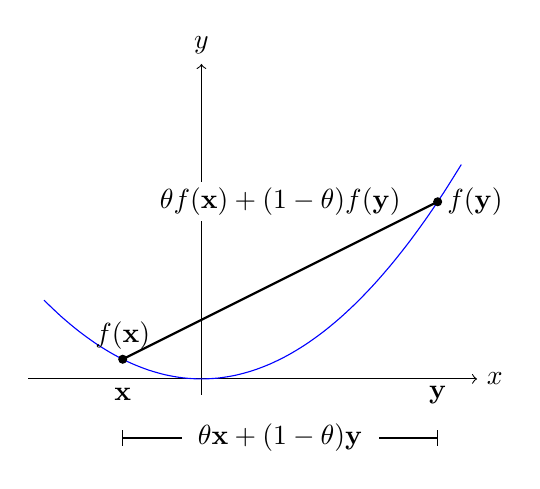
\begin{tikzpicture}
            \begin{scope}[shift={(-3,0)}]
                \draw[->] (-2.2,0) -- (3.5,0) node[right] {$x$};
                \draw[->] (0,-0.2) -- (0,4) node[above] {$y$};
                \draw[domain=-2:3.3,
                      smooth,
                      variable=\x,
                      blue] plot ({\x},{\x*\x/4});
                \fill[color=white] (-1,2) rectangle (2.75,2.5);
                \draw[fill=black] (-1,0.25) circle (0.05) node[above]{$f(\xx)$};
                \draw[fill=black] (3,2.25) circle (0.05) node[right]{$f(\yy)$};
                \draw (-1,-0.2) node {$\xx$};
                \draw (3,-0.2) node {$\yy$};
                \draw[thick] (-1,0.25) -- (3,2.25);
                \draw (1,2.25) node {$\theta f(\xx) + (1-\theta)f(\yy)$};
                \draw (1,-0.75) node {$\theta \xx + (1-\theta)\yy$};
                \draw (-1,-0.75) -- ++(0,0.1) -- ++(0,-0.2) -- ++(0,0.1) -- ++(0.75,0);
                \draw (3,-0.75) -- ++(0,0.1) -- ++(0,-0.2) -- ++(0,0.1) -- ++(-0.75,0);
            \end{scope}

            \begin{scope}[shift={(-3,0)}]
            \end{scope}
        \end{tikzpicture}
    \end{center}
    \caption{\textbf{Convex Functions}. This function $f : [a,b] \mapsto \RR$ is convex
    because it's domain is convex and every line between two points on the function lies
    above the function.}
    \label{fig:convex-function}
\end{figure}

\begin{definition}[Convex]
    Given a convex set $C$, a function $f : C \mapsto \RR$ is convex if,
    for $0\leq\theta\leq1$, given any $\xx,\yy\in C$,
    \[
        f(\theta\xx + (1-\theta)\yy) \leq \theta f(\xx) + (1-\theta)f(\yy).
    \]
\end{definition}

Intuitively, this means that a convex function always lies under a line
between any two points where it is evaluated. This is seen in Figure \ref{fig:convex-function}.

\begin{definition}[Concave Functions]
    Given a convex set $C$, function $f : C \mapsto \RR$ is concave
    if $-f$ is convex. That is, for $0\leq\theta\leq1$, given any $\xx,\yy\in C$,
    \[
        f(\theta\xx + (1-\theta)\yy) \geq \theta f(\xx) + (1-\theta)f(\yy).
    \]
\end{definition}

\begin{theorem}[Restriction To a Line]
    A function $f : \RR^n \mapsto \RR$ is convex if and only
    if $f$ is convex when restricted to any line that intersects
    its domain. Mathematically, $f$ is convex if and only if
    for all $x\in C$ and any $\vv\in\RR^n$ and $t\in\RR$,
    \[
        g(t) = f(\xx + t\vv)
    \]
    is convex where $g : \{t : \xx + t\vv \in C\} \mapsto \RR$
\end{theorem}
\begin{proof}
    Omitted. See \textit{Convex Optimization} by Boyd and Vandenberghe.
\end{proof}

\subsection{First Order Conditions: $f(x) \geq f(y) + \nabla f(y)^\T (x-y)$}

Generally speaking, determining convexity from the definition is
hard. In this section we will develop more tractable conditions that
will help us determine if an arbitrary function is convex. The following
necessary and sufficient condition for convexity is called the First Order
Condition because it relies only on the first derivative.

\begin{theorem}[First Order Conditions]
    Let $f$ be a function mapping from some convex set $C$ to $\RR$. Then
    $f$ is convex if and only if, given $\xx$ and $\yy$ from $C$,
    \[
        f(\xx) \geq f(\yy) + \nabla f(\yy)^\T (\xx - \yy).
    \]
\end{theorem}
\begin{proof}
    Omitted. See \textit{Convex Optimization} by Boyd and Vandenberghe.
\end{proof}

\subsubsection{Examples On Determining Convexity}

\begin{theorem}[Linear Functions are Both Concave and Convex]
    Given a function $f : C \mapsto \RR$ where $C$ is a convex
    set and for any $a,b\in\RR$ and $\xx,\yy\in\RR$
    \[
        f(a\xx + b\yy) = af(\xx) + bf(\yy),
    \]
    $f$ is both convex and concave. Note that $f$ is the definition
    of a linear function.
\end{theorem}
\begin{proof}
    Let $\xx,\yy$ be any elements of $C$ and $0\leq\theta\leq1$. Then
    by linearity
    \[
        f(\theta\xx + (1-\theta)\yy) = \theta f(\xx) + (1-\theta)f(\yy).
    \]
    Thus by definition $f$ is both convex and concave.
\end{proof}

\begin{example}
    $f(x) = x^2$ is convex.
\end{example}
\begin{proof}
    We will use the much more convenient second order condition
    for this problem later. Consider $x,y\in\RR$ and $0\leq\theta\leq1$.
    Then
    \begin{align*}
        f(\theta x + (1-\theta)y) &= (\theta x + (1-\theta)y)^2\\
        &= (\theta x + (1-\theta)y)(\theta x + (1-\theta)y)\\
        &= \theta^2x^2 + 2\theta(1-\theta)xy + (1-\theta)^2y^2.
    \end{align*}
    $f$ will be convex if and only if
    \[
        \theta f(x) + (1-\theta)f(y) - f(\theta x + (1-\theta)y) \geq 0
    \]
    for all $x,y$. We have
    \begin{align*}
        g = \theta f(x) + (1-\theta)f(y) - f(\theta x + (1-\theta)y) &= \theta x^2 + (1-\theta)y^2 - \theta^2x^2 - 2\theta(1-\theta)xy - (1-\theta)^2y^2\\
        &= \theta(1-\theta)x^2 - 2\theta(1-\theta)xy + \theta(1-\theta)y^2\\
        &= \theta(1-\theta)(x-y)^2
    \end{align*}
    We know $(x-y)^2 \geq 0$ for all $x$ and $y$. Similarly, when
    $\theta \in [0,1]$, both $\theta$ and $1-\theta$ are positive,
    so this expression is positive. Thus $f$ must be convex, as desired.
\end{proof}

\subsection{Second Order Conditions: $\nabla^2 f \succeq 0$}

Here we discuss the most useful condition for determining convexity.
\begin{theorem}[Second Order Conditions]
    A twice-differentiable function $f : C \mapsto \RR$ is convex if and
    only if and only if the Hessian
    \[
        \nabla^2 f \succeq 0
    \]
\end{theorem}
\begin{proof}
    Omitted.
\end{proof}

\subsubsection{More Examples On Determining Convexity}

\begin{example}[Quadratic Functions]
    The function $f : \RR^n \mapsto \RR$ defined by
    \[
        f(\xx) = \xx^\T A\xx + \bb^\T\xx + c
    \]
    is convex if $A \succeq 0$.
\end{example}
\begin{proof}
    We know
    \[
        \nabla^2 f = 2A.
    \]
    Similarly we know that $2A \succeq 0$ if and only if
    $A \succeq 0$. Thus by the second order conditions $f$
    is convex if and only if $A \succeq 0$.\\

    We can also show that $f$ is concave if $A\preceq 0$.
\end{proof}

\begin{example}
    $f(x) = a\;e^x$ is convex if $a \geq 0$.
\end{example}
\begin{proof}
    The Hessian
    \[
        \nabla^2f = \frac{d^2f}{dx^2} = a\;e^x \geq 0
    \]
    as long as $a\geq0$. Thus by the second order conditions
    $f$ is convex if $a\geq0$.
\end{proof}

\begin{example}
    The function $f : \RR^n \mapsto \RR$ defined by
    \[
        f(\xx) = e^{\xx^\T\xx} = e^{\xx_1^2 + \dots + \xx_n^2}
    \]
    is convex.
\end{example}
\begin{proof}
    Each element of the Hessian
    \[
        \nabla^2f_{ij} = \frac{\partial^2 f}{\partial x_i \partial x_j} = 4\xx_i\xx_j e^{\xx^\T\xx}.
    \]
    Therefore
    \[
        \nabla^2f = 4\xx\xx^\T e^{\xx^\T\xx}.
    \]
    Is this positive semidefinite? Consider $\zz\in\RR^n$. Then
    \[
        \zz^\T\nabla^2 f(x)\zz = \zz^\T4\xx\xx^\T e^{\xx^\T\xx} \zz = 4(\zz^\T\xx)^2 e^{\xx^\T\xx} \geq 0
    \]
    because $\exp(\cdot)$ and $(\zz^\T\xx)^2$ are both non-negative.
    Thus $\nabla^2f \succeq 0$ and by the second order conditions
    $f$ is convex.
\end{proof}

\subsection{Operations Preserving Convexity}

In this section we examine some handy tools for constructing
convex functions from other convex functions. There are \textit{many}
more properties than those shown here. See \textit{Convex Optimization}
by Boyd and Vandenberghe for many others.

\begin{theorem}[Non-Negative Weighted Sum]
    The function $F : C \mapsto \RR$ where $C$ is a convex set, $f_i : C\mapsto\RR$ is a convex
    function, $w_i \geq 0$ and
    \[
        F(\xx) = \sum_i w_i f_i(\xx)
    \]
    is convex.
\end{theorem}
\begin{proof}
    Let $\xx,\yy\in C$ and $0\leq\theta\leq1$. Then
    \begin{align*}
        F(\theta\xx + (1-\theta)\yy) &= \sum_i w_if_i(\theta\xx + (1-\theta)\yy)\\
        &\leq \sum_i w_i\left[ \theta f_i(\xx) + (1-\theta)f_i(\yy) \right]\\
        &= \theta F(\xx) + (1-\theta)F(\yy),
    \end{align*}
    as desired.
\end{proof}

\begin{theorem}[Pointwise Maximum]
    Given convex functions $f_i : C \mapsto \RR$, and $F : C \mapsto \RR$ defined
    as
    \[
        F(\xx) = \max_i f_i(\xx),
    \]
    $F$ is convex.
\end{theorem}
\begin{proof}
    By the definition of convexity, given $\xx,\yy\in C$ and $0\leq\theta\leq1$ we
    have
    \begin{align*}
        F(\theta\xx + (1-\theta)\yy) &= \max_i f_i(\theta\xx + (1-\theta)\yy)\\
        &\leq \max_i\{\theta f_i(\xx) + (1-\theta)f_i(\yy)\} \tag{because $f_i$ is convex}\\
        &\leq \theta \max_i f_i(\xx) + (1-\theta)\max_i f_i(\yy)\\
        &= \theta F(\xx) + (1-\theta) F(\yy),
    \end{align*}
    as desired.
\end{proof}

%%%%%%%%%%%%%%%%%%%%%%%%%%%%%%%%%%%%%%%%%%%%
\section{Optimization Problems}

An optimization problem is a problem of the form
\begin{align*}
    \text{minimize: } & f_0(\xx)\\
    \text{subj. to: } & f_i(\xx) \leq 0, \quad i=1,\dots,m\\
                      & h_i(\xx) = 0, \quad i=1,\dots,p
\end{align*}
where $f_0 : \RR^n \mapsto \RR$ is called the \textbf{objective function},
$f_i : \RR^n \mapsto \RR$ is an \textbf{inequality constraint}, and
$h_i : \RR^n \mapsto \RR$ is an \textbf{equality constraint}. The goal of
an optimization problem, as you might be able to guess, is to find $\xx$ in
the problem domain domain 
\[
    \Dc = \bigcap_{i=0}^m\mathbf{dom}\; f_i \;\cap\; \bigcap_{i=1}^p \mathbf{dom}\; h_i
\]
that minimizes $f_0(\xx)$ subject to the given conditions. The problem is
said to be \textit{feasible} if such an $\xx$ exists, and \textit{infeasible}
otherwise.\\

The optimal value $p^\star$ of the problem above is defined to be
\[
    p^\star = \inf\{f_0(\xx) : f_i(\xx) \leq 0,\; i=1,\dots,m,\; h_i(\xx)=0,\, i=1,\dots,p\}.
\]
If there are feasible points $\xx_k$ with $f_0(\xx_k)\to -\infty$ as
$k\to\infty$, then we say the problem is \textit{unbounded below}.\\

Note that we could have a similarly defined \textit{maximization} problem.
Everything is the same except for the definition of \textit{unbounded below},
obviously.

\subsection{Optimal Points}

We say $\xx^\star$ is an \textit{optimal point} (or that it solves the
above problem) if $\xx^\star$ is feasible and $f_0(\xx^\star)=p^\star$.
If an optimal point exists, we say the problem is \textit{solvable}.\\

We say a feasible point $\xx$ is \textit{locally optimal} if there exists
some $R > 0$ such that $\xx$ solves

\begin{align*}
    \text{minimize: } & f_0(\zz)\\
    \text{subj. to: } & f_i(\zz) \leq 0, \quad i=1,\dots,m\\
                      & h_i(\zz) = 0, \quad i=1,\dots,p\\
                      & || \zz - \xx ||_2 \leq R
\end{align*}
for variable $\zz$. This intuitively means that $\xx$ minimizes
$f_0$ over nearby points in the feasible set.

\subsection{Equivalent Problems}

Given an optimization problem of the form
\begin{align*}
    \text{minimize: } & f_0(\xx)\\
    \text{subj. to: } & f_i(\xx) \leq 0, \quad i=1,\dots,m\\
                      & h_i(\xx) = 0, \quad i=1,\dots,p
\end{align*}
we may want to express our problem in a cleaner or easier
to solve form. Under certain conditions changing our problem's
form will not actually change the solution. Note that, as usual,
there are a few more possible transformations that are kosher.
Check out Boyd and Vandenberghe for these, but the ones shown here
are likely the only ones you will need.

\subsubsection{Scaling}

The problem
\begin{align*}
    \text{minimize: } & \alpha_0f_0(\xx)\\
    \text{subj. to: } & \alpha_if_i(\xx) \leq 0, \quad i=1,\dots,m\\
                      & \beta_ih_i(\xx) = 0, \quad i=1,\dots,p
\end{align*}
for $\alpha > 0$ and $\beta \neq 0$ is equivalent to the original
problem. This should be intuitive since, for example $x^2$ is minimized
at 0, changing the scale of your axes maintains that minimum. Similarly,
if equality holds (ie. $4x+2=0$) multiplying by any non-zero number on
both sides maintains that equality.

\subsubsection{Change of Variables}

Given an one-to-one mapping $\phi : \RR^n \mapsto \RR^n$, where the image
(range) of $\phi$ covers the domain of your problem $\Dc$, the problem
\begin{align*}
    \text{minimize: } & f_0(\phi(\xx))\\
    \text{subj. to: } & f_i(\phi(\xx)) \leq 0, \quad i=1,\dots,m\\
                      & h_i(\phi(\xx)) = 0, \quad i=1,\dots,p
\end{align*}
is equivalent to the original. This should be clear. If $x$ solves the
original problem, then $z = \phi^{-1}(x)$ solves the transformed problem.
The converse also holds.

\subsubsection{Transformation of Objective and Constrain Functions}

Suppose $\psi_0 : \RR \mapsto \RR$ is monotonically increasing, $\phi_1,\dots,
\psi_m : \RR \mapsto \RR$ satisfy $\phi_i(u) \leq 0$ if and only if $u \leq 0$,
and $\psi_{m+1},\dots,\phi_{m+p} : \RR\mapsto\RR$ satisfy $\phi_i(u)=0$ if and only
if $u=0$. The problem
\begin{align*}
    \text{minimize: } & \psi_0(f_0(\xx))\\
    \text{subj. to: } & \psi_i(f_i(\xx)) \leq 0, \quad i=1,\dots,m\\
                      & \psi_{m+i}(h_i(\xx)) = 0, \quad i=1,\dots,p
\end{align*}
is equivalent to the original. This should be evident from the conditions
we placed on each $\psi_j$.

\subsubsection{Slack Variables}

This will come in very handy. A prudent observation is that $f_i(x)\leq 0$
if and only if for some $s_i \geq 0$, $f_i(x) + s_i = 0$. Thus the problem
\begin{align*}
    \text{minimize: } & f_0(\xx)\\
    \text{subj. to: } & f_i(\xx) + s_i = 0, \quad i=1,\dots,m\\
                      & h_i(\xx) = 0, \quad i=1,\dots,p\\
                      & s_i \geq 0, \quad i=1,\dots,m
\end{align*}
is equivalent to the original.

\subsubsection{Epigraph Form}

The \textit{epigraph form} of the original problem is
\begin{align*}
    \text{minimize: } & t\\
    \text{subj. to: } & f_0(\xx) - t \leq 0,\\
                      & f_i(\xx) \leq 0, \quad i=1,\dots,m\\
                      & h_i(\xx) = 0, \quad i=1,\dots,p
\end{align*}
where $t\in\RR$. It should be clear that this is the same as the original
problem as the first constraint can be viewed as $f_0(\xx) \leq t$. Thus
the objective must always lie under $t$ and minimizing $t$ will minimize the
highest possible value of $f_0$.

\subsection{Convex Optimization Problems}

We will now study the branch of optimization problems we will see
\textit{extremely} often in our studies. We say a problem of the
form

\begin{align*}
    \text{minimize: } & f_0(\xx)\\
    \text{subj. to: } & f_i(\xx) \leq 0, \quad i=1,\dots,m\\
                      & A\xx = \bb
\end{align*}

is a \textbf{convex optimization problem} if the objective function
and inequalities $f_i$ are convex, and the equality constraints
$h_i$ are linear. Convex problems are, as a whole, extremely \textit{nice}
in the sense that we have efficient (read `polynomial time') algorithms
for finding global optima.\\

At heart, a convex optimization problem is 
just a minimization of a convex function within a convex domain.


\subsubsection{Global Optimality of a Convex Optimum}

The reason that convex optimization problems are so nice to solve
is that \textit{any} optimum is a global optimum. In other words,
if you find some solution you find \textit{the} solution. This is
by no means the case in non-convex problems such as neural networks,
although you might use similar methods to find \textit{sufficiently
good solutions}.

\begin{theorem}[Global Optimality]
    Given a convex optimization problem, and local optimum $\xx^\star$
    such that
    \[
        f_0(\xx) = \inf\{f_0(\zz) : \zz\text{ feasible and } ||\zz-\xx||_2 \leq R\}
    \]
    for some $R > 0$. $\xx^\star$ is the global optimum.
\end{theorem}
\begin{proof}
    (Boyd)
    Suppose such a problem and local optimum. Now suppose, to the
    contrary, that $\xx$ is \textit{not} the global optimum,
    and therefore there exists some feasible $\yy$ such that $f_0(\yy)
    < f_0(\xx)$. Then $||\yy-\xx||_2 >R$ because otherwise $f_0(\xx)
    \leq f_0(\yy)$. Consider a point $\zz$ given by
    \[
        \zz = (1-\theta)\xx+ \theta\yy \quad\text{and}\quad \theta=\frac{R}{2||\yy-\xx||_2}.
    \]
    Then $||\xx-\zz||_2=R/2 < R$. By convexity of the feasible set,
    $\zz$ is feasible. By the convexity of the objective function $f_0$
    we also have
    \[
        f_0(\zz) \leq (1-\theta)f_0(\xx) + \theta f_0(\yy) < f_0(\xx),
    \]
    contradicting our assumption of local optimality. Thus $\xx$
    must be the global optimum ($R\to\infty$).
\end{proof}

\subsubsection{Linear Programs}

While we won't study Linear Programs much in the course, they
are necessary to understand and are a central tool in operations
research and graph algorithms. A linear program is a convex
optimization problem of the form
\begin{align*}
    \text{minimize: } & \cc^\T\xx\\
    \text{subj. to: } & G\xx \leq \hh,\\
                      & A\xx = \bb
\end{align*}
where $G\in\RR^{m\times n}$ and $A\in\RR^{p\times n}$. Note that
because the objective function is linear this could also have been
a maximization problem with no change to convexity. For a ton
of interesting applications, see Boyd and Vandenberghe, or consider
taking the Operations Research Course!

\subsubsection{Quadratic Programs}

Interestingly enough, of all standard convex optimization problem classes,
quadratic programs seem to come up the most in machine learning. Basically,
pay attention!\\

A quadratic program is an optimization program of the form
\begin{align*}
    \text{minimize: } & \frac{1}{2}\xx^\T P\xx + \qq^\T\xx + \rr\\
    \text{subj. to: } & G\xx \preceq\hh\\
                      & A\xx = \bb
\end{align*}
where $P\in\SS_+^n$, $G\in\RR^{m\times n}$, and $A\in\RR^{p\times n}$.
In this class of program, we are minimizing a quadratic function inside
of a polyhedron.

\subsection{Examples of Convex Optimization Problems}

Here we present two examples of applied convex optimization
problems. See \textit{Convex Optimization} by Boyd \&
Vandenberghe for many, many more.

\subsubsection{Analytic Centering}

Consider the problem of finding the `center' of some
polygon $\{\xx : A\xx \preceq \bb\}$. We first need to denote
what we consider the optimal center. The \textit{Chebyshev Center}
of a set of points $\{\xx_i\}$ is the center of the smallest
circle that will fit around all of the points. This is easily
expressed as the following optimization problem:
\begin{align*}
    \text{minimize: } & r\\
    \text{subj. to: } & ||\xx_i - \cc||_r \leq r\\
\end{align*}
where $r$ and $\cc$ are variables. This is obviously convex.
We could set $\xx_i$ as the vertices of the polygon to then find a
center. But that has some issues, for example, when your polygon
is a very long, thin rectangle with a triangle slapped onto one side
of it. The Chebyshev Center won't include be affected by the triangle
at all until it hits the end of the circle. To remedy this issue we
will consider a more effective method of finding the center below.\\

What if we wanted to create
a \textit{unconstrained} convex optimization problem that would
given us some definition of a `center'? First note that $A\xx \preceq \bb$
implies that $a_i^\T\xx \leq \bb_i$ where $a_i$ is the $i-$th row
of $A$. This condition is satisfied, obviously, when $-\log (\bb_i - a_i^\T\xx)$
exists. But more importantly, as $a_i^\T\xx$ approaches $\bb_i$, we
note that the $-\log$ term approaches infinity. This is called a
`$\log$ barrier'. Now if we combine a bunch of $\log$ barriers, say,
perhaps, along each of the edges of our polygon and ``walking down
hill'' until we find the point that minimizes all of the log barriers. This
sounds, intuitively like a good idea of a `center', and is called the
\textit{Analytic Center} of a polygon. This is also easily expressed as
a convex optimization problem, this time without constraints:
\begin{align*}
    \text{minimize: } f_0(\xx) = -\sum_{i}\log(\bb_i - a_i^\T\xx)\\
\end{align*}
Note that the gradient
\[
    \nabla f_0 = \sum_i\frac{\aa_i}{\bb_i - \aa_i^\T\xx},
\]
so if you are `far' from a barrier it doesn't effect your gradient. This
can be fed into any standard gradient based optimizer, as seen in Figure
\ref{fig:analytic-center}\\

Now let's show that the analytic centering problem is convex. First, note
that $\log$ is a concave function (check this for yourself), so $-\log$ is
convex. Second, as affine composition $f(A\xx + \bb)$ preserves convexity,
$-\log(b_i - a_i^\T\xx_i)$ is also convex. Finally, as a non-negative weighted
sum of convex functions, the final objective $f_0$ is therefore convex.

\begin{figure}
    \centering
    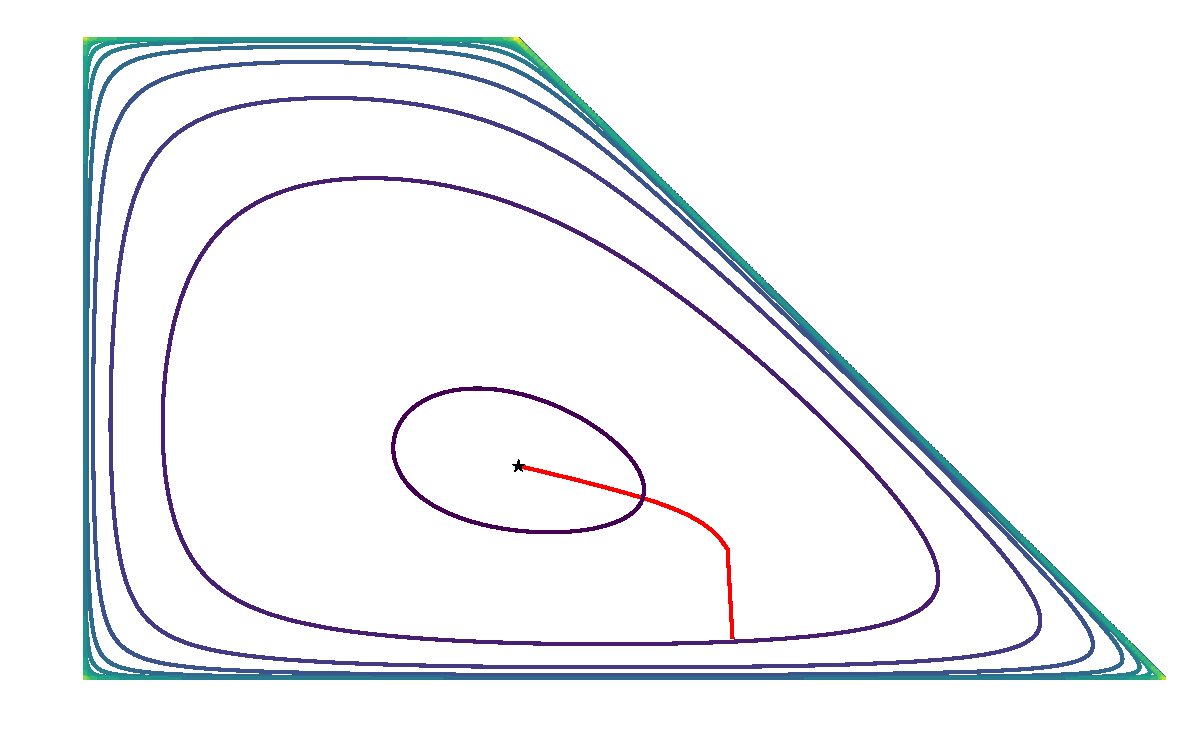
\includegraphics[width=0.6\linewidth]{fig/analytic_centering.pdf}
    \caption{\textbf{Analytic Centering}. Here we compute the analytic center
    of a polygon in $\RR^2$. Contour lines represent the objective surface
    while the red path represents the progression of gradient descent. The
    star is the optimal center. See \url{https://math189r.github.io/materials/section/fig_code/analytic_centering.py}
    for code to generate this plot.}
    \label{fig:analytic-center}
\end{figure}


\subsubsection{Logistic Regression}

Note that our notation will assume $\xx_0=1$ as a bias term.\\

Now let's reconsider logistic regression as an optimization problem.
Suppose we have a bunch of points $\xx_i$, with labels $\yy_i \in \{0,1\}$.
We want to classify some new point $\xx$.
Now suppose we generate a distribution over the labels of a given point
$\xx$ with
\[
    \PP(\yy = 1 | \xx,\thetab) = \sigma(\thetab^\T\xx) = \frac{1}{1 + e^{-\thetab^\T\xx}} \in (0,1).
\]
Intuitively, this takes regular linear regression over the binary labels
$\{0,1\}$ and squashes it into a function $f : \RR \mapsto [0,1]$ to give
us the ability to probabilistically interpret the output of our classifier.
In a frequentist setting we want to maximize the \textit{likelihood} of our data,
that is, the probability of our labelled data given our parameters (just
$\thetab$ in this case). However, because the actual likelihood will involve
products we can transform into log space (because $\log(x)$ is a monotonically
increasing function!!!) and equivalently maximize the log likelihood
\[
    \Lc(\thetab) = \sum_{i=1}^m \log \PP(\yy=\yy_i | \xx_i, \thetab) = \sum_{i=1}^m \log \begin{cases}
        \sigma(\thetab^\T\xx) & \text{if $\yy_i=1$}\\
        1-\sigma(\thetab^\T\xx) & \text{if $\yy_i=0$}
    \end{cases}
\]
Note that due to the binary labels we can represent this compactly as
\[
    \Lc(\thetab) = \sum_{i=1}^m \yy_i\log(\sigma(\thetab^\T\xx)) + (1-\yy_i)\log(1-\sigma(\thetab^\T\xx)).
\]
Now our (unconstrained) optimization problem becomes simply
\begin{align*}
    \text{maximize: } \Lc(\thetab)
\end{align*}
where we could add a $\lambda \thetab^\T\thetab$ regularization term if we place
a Gaussian prior on our parameter vector $\thetab$. Usually this would be a
good idea.\\

Now to optimize this, as we will/have seen, first note that the derivative of
the sigmoid function $\sigma'(x) = \sigma(x)\left(1-\sigma(x)\right)$. Then the
gradient of our log output $\log\PP(\yy=1|\xx,\thetab) = \log\sigma(\thetab^\T\xx)$
becomes
\[
    \nabla_\theta \log\sigma(\thetab^\T\xx) = \xx(1-\sigma(\thetab^\T\xx) ).
\]
Similarly,
\[
    \nabla_\theta \log(1-\sigma(\thetab^\T\xx)) = -\xx\sigma(\thetab^\T\xx).
\]

Prove to yourself why this is correct. Thus the derivative of our objective $\Lc(\thetab)$
becomes
\[
    \nabla_\theta \Lc = \sum_{i=1}^m \left[  \yy_i(1-\sigma(\thetab^\T\xx)) - (1-\yy_i)\sigma(\thetab^\T\xx)  \right]\xx_i = \sum_{i=1}^m \left[ \yy_i - \sigma(\thetab^\T\xx) \right]\xx.
\]
This can be input into any standard gradient-based optimization algorithm.\\

Now let's show that logistic regression is convex. This is equivalent to showing
the objective function $f_0$ is concave, as we are maximizing. As affine composition
$f(A\xx+\bb)$ and non-negative weighted summation preserve concavity, one can
see that this is the same as showing that
\[
    f(x) = \log\sigma(x)
\]
is concave on $\RR$. As $\sigma'(x)=\sigma(x)(1-\sigma(x))$, we can see that
\[
    f'(x) = \frac{\sigma(x)(1-\sigma(x))}{\sigma(x)} = 1-\sigma(x)
\]
and
\[
    f''(x) = -\sigma(x)(1-\sigma(x)),
\]
which always negative, because $\sigma(x)\in[0,1]$. Thus the objective and
therefore the whole problem of logistic regression is convex, as desired.

%%%%%%%%%%%%%%%%%%%%%%%%%%%%%%%%%%%%%%%%%%%%
\section{Algorithms for Solving Convex Problems}

As has been the theme thus far, if you want to see \textit{much} more information
about algorimths for solving convex optimization problems, see \textit{Convex Optimization}
by Boyd \& Vandenberghe. Here we will just revisit good old gradient descent
and Newton's Method for solving unconstrained convex optimization problems.
Boyd goes into detail on solving constrained optimization problems efficiently,
but we likely won't need to do much of that (hopefully!).

\begin{figure}
    \centering
    \begin{center}
        \begin{tikzpicture}
            \begin{scope}[shift={(-3.5,0)}]
                \draw[->] (-2.2,0) -- (3.5,0) node[right] {$x$};
                \draw[->] (0,-0.2) -- (0,4) node[above] {$y$};
                \draw[domain=-2:3.3,
                      smooth,
                      variable=\x,
                      blue] plot ({\x},{exp(\x/5)*\x*\x/4});
                \draw (2,0) node[below]{$\xx_0$};
                \draw[color=black!30] (2,0) -- (2,{exp(2/5)});
                \draw[thick,-stealth] (2,1.49) -- ++(0.75,{1.79*0.75}) node[right] {$\nabla f(x_0)$};
                \draw (-1,0) node[below]{$\xx_1$};
                \draw[color=black!30] (-1,0) -- (-1,{exp(-1/5)/4});
                \draw (-1,-0.75) -- ++(0,0.1) -- ++(0,-0.2) -- ++(0,0.1) -- ++(0.5,0);
                \draw (2,-0.75) -- ++(0,0.1) -- ++(0,-0.2) -- ++(0,0.1) -- ++(-0.5,0);
                \draw (0.5,-0.75) node {$-\eta\nabla f(\xx_0)$};
            \end{scope}
            \begin{scope}[shift={(3.5,0)}]
                \draw[->] (-2.2,0) -- (3.5,0) node[right] {$x$};
                \draw[->] (0,-0.2) -- (0,4) node[above] {$y$};
                \draw[domain=-2:3.3,
                      smooth,
                      variable=\x,
                      blue] plot ({\x},{exp(\x/5)*\x*\x/4});
                \draw[domain=-1.5:3.3,
                      smooth,
                      variable=\x,
                      red!75] plot ({\x},{1.49182 + 1.79019*(\x-2) + 0.701158*(\x-2)*(\x-2)});
                \draw (2,0) node[below] {$\xx_0$};
                \draw[color=black!30] (2,0) -- (2,1.49182);
                \draw (0.723404,0) node[below] {$\xx_1$};
                \draw[color=black!30] (0.723404,0) -- (0.723404,0.34915);
                \draw (0.723404,-0.5) -- ++(0,-0.1) -- ++({2-0.723404},0) -- ++(0,0.1);
                \draw ({(2+0.723404)/2},-0.65) node[below] {$-\nabla^2f(\xx_0)^{-1}\nabla f(\xx_0)$};
            \end{scope}
        \end{tikzpicture}
    \end{center}
    \caption{\textbf{Optimization Algorithms}. A vizualization of gradient
    descent and Newton's Method. Newton's Method, although you can't tell
    much in this example, is much faster. While Newton's Method analtyically
    solves a quadratic approximation of your (hopefully convex) problem at each
    iteration, gradient descent acts as an approximation of that, just taking
    small steps in the right direction to optimize your problem. If the learning
    rate $\eta$ is too large, your iterates will start to diverge. If your learning
    rate is too small, your iterates will take too long to converge.}
    \label{fig:optimization-algorithms}
\end{figure}

\subsection{Gradient Descent}

Suppose, given $f : \RR^n \mapsto \RR$, we want to find when $f'(\xx)=0$.
Note that while $f$ need not be convex, if $f$ is convex we are guarenteed
to find the global optimum when we find a critical point. Now picture our function
as a surface mapping $\RR^2$ to $\RR$. Intuitively, if we want to minimize
$f$, we just need to walk in the direction of `down hill'. Assuming $f$ is
once-differentiable, we can use the gradient $\nabla f$ to define this direction.
So, given a starting point, we need to take steps in the direction of $\nabla f$
of some size, called the learning rate $\eta$. We do this until our gradient
$\nabla f$ is smaller than some $\epsilon$.

\IncMargin{1em}
\begin{algorithm}
    \SetKwInOut{Input}{input}\SetKwInOut{Output}{output}
    \textbf{Gradient Descent}\\
    \Input{$f$, $\nabla f$, $\eta(t)$, starting point $\xx_0$, tolerance $\epsilon$}
    \Output{optimal point $\xx^\star$}
    $t \leftarrow 0$\\
    \While{$|| \nabla f ||_2 \geq \epsilon$}{
        $\xx_{t+1} \leftarrow \xx_t - \eta(t)\nabla f(\xx_t)$\\
        $t \leftarrow t + 1$
    }
    \textbf{return } $\xx^\star = \xx_{t+1}$
\end{algorithm}

Oftentimes you can use a contant $\eta(t) = 0.01$ or some similarly small number.
More sophisticated learning rates and augmentation terms, like adding a \textbf{momentum
term} giving an update
\[
    \xx_{t+1} \leftarrow \xx_t - \eta(t)\nabla f(\xx_t) + \mu_t(\xx_t - \xx_{t-1})
\]
where $\mu_t$ might be a constant around $0.9$. You can get a sense of how heuristic these
methods are!
Some problems with gradient descent are that
\begin{itemize}
    \item it is slow in convergence compared to second order methods
    \item it provides a number of hyperparameters to set, which can
        end up using a lot of heuristic based approaches to improvement
    \item if your problem isn't ``round'' (think $\xx^\T\xx$ where the
        axes are scaled the same) you will end up zig-zagging along a
        basin. Newton's method remedies this by being scale invariant
\end{itemize}

\subsubsection{Minibatch and Stochastic Gradient Descent}

Often times in machine learning specifically we will have huge datasets
and objective functions of the form
\[
    f_0(\theta) = \frac{1}{m}\sum_{i=1}^m f(\xx_i | \theta)
\]
where $\xx_i$ are our training examples and $f(\xx|\theta)$ is our loss function.
In this case, $m$ is so large (ie. $m > 10^5$ or $m > 10^6$) that attempting to compute
\[
    \nabla f_0 = \frac{1}{m}\sum_{i=1}^m \nabla f(\xx_i | \theta)
\]
at every iteration of training using gradient descent would be too slow. Intuitively,
if you use (batch, like above) gradient descent you have to go through your
entire training set each iteration. If you have a million points, however,
the last point $i=m$ will hardly give you any information on average about the surface
you are on. Thus, a natural approximation is to select a random subset of size
$k$ at each iteration and use those $k$ points to compute an approximated gradient
\[
    \nabla f_0 \approx \frac{1}{k}\sum_{i=1}^k \nabla f(\xx_i | \theta)
\]
and use that to compute the update. 

\IncMargin{1em}
\begin{algorithm}
    \SetKwInOut{Input}{input}\SetKwInOut{Output}{output}
    \textbf{Stochastic Gradient Descent}\\
    \Input{$f$, $\nabla f$, $\eta(t)$, starting point $\thetab_0$, dataset $\Dc$, tolerance $\epsilon$, batch size $k$}
    \Output{optimal point $\thetab^\star$}
    $t \leftarrow 0$\\
    \While{$|| \nabla f ||_2 \geq \epsilon$}{
        select training points $X = \{\xx_i\}_{i=1}^k\subseteq \Dc$ at random\\
        $\thetab_{t+1} \leftarrow \thetab_t - \eta(t)\nabla f(X | \thetab_t)$\\
        $t \leftarrow t + 1$
    }
    \textbf{return } $\thetab^\star = \thetab_{t+1}$
\end{algorithm}

With different values of $k$ this algorithm is called different things. The algorithm
is theoretically guarenteed to converge for any $k$ under certain conditions on hyperparameters.
\begin{itemize}
    \item $k=1$ (Stochastic Gradient Descent): You might think this wouldn't
        do too well because you lose so much information by only looking at a
        single point but it is actually used heavily in distributed model learning
        due to its algorithmic simplicity.
    \item $1 < k < m$ (Minibatch Gradient Descent): This is the de-facto standard
        for solving large problems (well, with small variants to the update). Usually in Deep
        Learning people set $15 < k < 256$ with $k=128$ being pretty standard.
    \item $k=m$ This is just regular (batch) gradient descent as seen above.
\end{itemize}

\subsection{Newton's Method}

Here we introduce a method that is \textit{super fast} but probably won't scale
to problems with more than a couple thousand variables depending on your
problem structure. Effectively Newton's Method does the following logic:
\begin{enumerate}
    \item We want to minimize a twice-differentiable function $f : \RR^n \mapsto \RR$. We have an
        initial guess for the minimizer $\xx_0$.
    \item We know how to minimize quadratic systems $\xx^\T A\xx + \bb^\T\xx + \cc$
        in closed form. Generally speaking this is the best approximator to our function
        that we can optimize in closed form.
    \item Why don't we take your function and approximate it as a quadratic Taylor
        polynomial about your guess and set your guess to be the optimum of that
        approximation?
\end{enumerate}
See Figure \ref{fig:optimization-algorithms} for a visualization of a Newton step. Note 
that, about some $\xx_0$, the quadratic Taylor approximation
\[
    \widetilde f(\xx) = f(\xx_0) + \nabla f(\xx_0)^\T(\xx - \xx_0) + \frac{1}{2}(\xx-\xx_0)^\T\nabla^2 f(\xx_0)(\xx-\xx_0)
\]
with gradient vanishing when
\[
    \nabla f(\xx) = \nabla f(\xx_0) + \nabla^2 f(\xx_0)(\xx-\xx_0) = 0,
\]
or
\[
    \xx = \xx_0 - \nabla^2 f(\xx_0)^{-1} \nabla f(\xx_0).
\]
Note that this looks strikingly similar to gradient descent, except instead of having
a scalar learning rate we have the inverse of a linear map $\nabla^2 f(\xx_0)^{-1}$.
Also, solving that system
\[
    \nabla^2f(\xx_0)\dd = \nabla f(\xx_0)
\]
is what calls for trouble when trying to optimize at very large scale.
Many approximation algorithms exist (see L-BFGS for an example) to work
in first order methods yet approximate the second order terms during optimization.
For many problems there exists a helpful structure in the Hessian (eg. tridiagonal
or arrow structure) you can exploit to solve that system relatively quickly. In
general using a backslash solver (\texttt{A$\setminus$b}) is a terrible idea for
using Newton's Method to optimize at scale because of this, but it is much preferred
to using \texttt{pinv(A)*b} or \texttt{inv(A)*b}. If $f$ is just convex, for example you can use a
Cholesky decomposition to cut the backslash time in half.

\IncMargin{1em}
\begin{algorithm}
    \SetKwInOut{Input}{input}\SetKwInOut{Output}{output}
    \textbf{Newton's Method}\\
    \Input{$f$, $\nabla f$, $\nabla^2f$, starting point $\xx_0$, tolerance $\epsilon$}
    \Output{optimal point $\xx^\star$}
    $t \leftarrow 0$\\
    \While{$|| \nabla f ||_2 \geq \epsilon$}{
        solve $\nabla^2 f(\xx_t) \dd_t = \nabla f(\xx_t)$ for $\dd_t$\\
        $\xx_{t+1} \leftarrow \xx_t - \dd_t$\\
        $t \leftarrow t + 1$
    }
    \textbf{return } $\xx^\star = \xx_{t+1}$
\end{algorithm}

The reason Newton's Method is fast is because it obeys what is called \textbf{quadratic
convergence}. Roughly speaking, once your iterates $\xx_t$ get close enough to the optimum,
every iteration will double the number of digits you are precise to. This means that once
you have a pretty accurate answer, running for one or two more iterations will max out
double floating point precision on any computer. Even when you aren't in the quadratic region,
Newton's Method's number of iterations to become $\epsilon$ suboptimal is still bounded above
by
\[
    \frac{f(\xx_0)-p^\star}{\gamma} + \log_2\log_2(1/\epsilon) \tag{$\log_2\log_2(1/\epsilon)\approx6.$}
\]
where $\gamma$ is a constant depending on the problem. Usually $1/\gamma$ is about $375$,
depending on the problem, but Newton's Method empirically converges much faster than even
that bound. See Boys \& Vandenberghe for a proof of this bound.

%%%%%%%%%%%%%%%%%%%%%%%%%%%%%%%%%%%%%%%%%%%%
\section{Duality}

The idea of ``duality'', forming a complementary problem that maintains
all of the information of your problem, is found all over mathematics.
In optimization as a whole, and convex optimization specifically, duality
is central. First we will investigate an intuitive representation of any
constrained convex optimization problem which will then lead us directly to
Lagrange Duality before investigating the implications of this.

\subsection{Constructing The Dual}

Given an optimization problem (which we will call the \textbf{primal problem})
\begin{align*}
    \text{minimize: } & f_0(\xx)\\
    \text{subj. to: } & f_i(\xx) \leq 0, \quad i=1,\dots,m\\
                      & h_i(\xx) = 0, \quad i=1,\dots,p
\end{align*}
note that minimizing $f_0$ under the constraints is the same
as optimizing $f_0$ over all of $\RR^n$ while letting
\[
    f_0(\xx) = \begin{cases}
        f_0(\xx) & \text{if constraints are satisfied}\\
        \infty   & \text{otherwise.}
    \end{cases}
\]
This makes sense, because if there is any feasible point, there will
exist $f_0(\xx_{feasible}) < \infty$ if there is any practical solution
to your problem. Otherwise, if $f_0(\xx_{feasible}) = \infty$, you have
still solved your problem! The question now is how to change our constrained
optimization problem into an unconstrained one by embedding the constraints
in the objective. One simple way might be to use an indicator function
\[
    I_-(u) = \begin{cases}
        0      & \text{if $u \leq 0$}\\
        \infty & \text{if $u > 0$}
    \end{cases}
\]
to wrap each inequality constraint, so that if at any $\xx$ any $f_i(\xx) > 0$,
the objective will rise to infinity. Convince yourself why this would work.
Similarly, for equality constraints, if we use another indicator function
\[
    I_0(u) = \begin{cases}
        0      & \text{if $u = 0$}\\
        \infty & \text{otherwise}
    \end{cases}
\]
to wrap each equality, we can assure that our objective diverges to infinity if
at any $\xx$ we have $h_i(\xx) \neq 0$. Our problem then becomes
\begin{align*}
    \text{minimize: } & f_0(\xx) + \sum_{i=1}^m I_-(f_i(\xx)) + \sum_{i=1}^p I_0(h_i(\xx)).
\end{align*}
Convince yourself why this is the same. You can intuitively think of the indicator
functions as expressing a ``hard displeasure'' to the objective whenever constraints
are not satisfied. To solve anything tractably a natural step might be to approximate
this ``hard displeasure function'' with a ``soft'', linear displeasure function
\[
    I_-(u) \approx \lambda u\text{ for $\lambda \geq 0$} \qquad I_0(u) \approx \nu u \text{ for unconstrained $\nu$}.
\]
You can immediately see that these linear approximations are not the same, but are
always underestimates of the hard indicators. See Figure \ref{fig:dual-vars}.
Representing our problem in this new way we have an objective
\begin{align*}
    \text{minimize: } & L(\xx,\lambdab, \nub) = f_0(\xx) + \sum_{i=1}^m \lambda_i f_i(\xx) + \sum_{i=1}^p \nu_i h_i(\xx)\\
    \text{subj. to: } & \lambdab \succeq 0.
\end{align*}
We call $L(\xx,\lambdab, \nub)$ the \textbf{Lagrangian} of our optimization problem.
As our linear approximation of the indicator functions are always below these functions,
we might see that our primal problem is \textit{exactly}
\[
    p^\star = \inf_\xx \sup_{\nu; \lambda \geq 0} L(\xx,\lambdab,\nub)
\]
The \textbf{dual} of our problem is just the flip of order with which we are
optimizing, namely the dual
\[
    d^\star = \sup_{\nu; \lambda \geq 0} \inf_\xx L(\xx,\lambdab,\nub).
\]

\begin{figure}
    \centering
    \begin{center}
        \begin{tikzpicture}
            \begin{scope}[shift=({-4,0})]
                \draw[->] (-2.2,0) -- (3.5,0) node[right] {$u$};
                \draw[->] (0,-0.2) -- (0,4) node[above] {$y$};
                \draw[very thick] (-2.2,0) -- (0,0);
                \draw[fill=black] (0,0) circle (0.07);
                \draw[dashed, very thick] (0,3.5) -- (3.5,3.5) node[right] {$I_-(u)$};
                \draw[fill=white] (0,3.5) circle (0.07);
                \draw (0,3.5) node[left] {$\infty$};
                \draw[color=blue] (-1,{0.5*-1}) -- (3.5,{0.5*3.5});
                \draw (3.5,{0.5*3.5+0.1}) node[right] {$\lambda u$};
            \end{scope}
            \begin{scope}[shift=({4,0})]
                \draw[->] (-2.2,0) -- (3.5,0) node[right] {$u$};
                \draw[->] (0,-0.2) -- (0,4) node[above] {$y$};
                \draw[fill=black] (0,0) circle (0.07);
                \draw[dashed, very thick] (-2,3.5) -- (3.5,3.5) node[right] {$I_0(u)$};
                \draw[fill=white] (0,3.5) circle (0.07);
                \draw (-0.5,3.5) node[above] {$\infty$};
                \draw[color=red] (-1,{0.75*-1}) -- (3.5,{0.75*3.5});
                \draw (3.5,{0.75*3.5+0.1}) node[right] {$\nu u$};
            \end{scope}
        \end{tikzpicture}
    \end{center}
    \caption{\textbf{Constrain Indicator Approximation:} So long as $\lambda > 0$ with $\nu \lessgtr 0$,
    $\lambda u \leq I_-(u)$, and $\nu u \leq I_0(u)$. This lets us construct the
    dual in a more tractable manner.}
    \label{fig:dual-vars}
\end{figure}

\subsection{Duality Gap: $p^\star - d^\star$}

As we discussed, the linear approximation of our constraints is always an under approximation,
so if we don't maximize that first our problem is always an under approximation of our primal
problem. Thus we have the following theorem:

\begin{theorem}[Weak Duality]
    For \textit{any} optimization problem (even a non-convex one),
    \[
        d^\star \leq p^\star.
    \]
\end{theorem}
\begin{proof}
    See discussion above.
\end{proof}

From this we can create a handy definition.
\begin{definition}[Duality Gap]
    We define the \textbf{duality gap} to be
    \[
        p^\star - d^\star \geq 0.
    \]
\end{definition}
As the duality gap tends towards $0$ it means our dual better and better approximates
our primal problem. In some (any many we will see) cases, $p^\star = d^\star$. In this
case we say \textbf{strong duality} holds, and solving the dual is equivalent to solving
the primal problem. In general this is not the case, but if the problem is convex,
ie. of the form
\begin{align*}
    \text{minimize: } & f_0(\xx)\\
    \text{subj. to: } & f_i(\xx) \leq 0, \quad i=1,\dots,m\\
                      & A\xx = \bb
\end{align*}
with $f_i$ convex, we usually (but not always) will have strong duality. One sufficient
but not necessary condition for strong duality is \textbf{Slater's Condition}.

\begin{theorem}[Slater's Condition]
    If the primal problem is convex as above, and there exists some $\xx\in \mathrm{relint} \;\Dc$
    such that
    \[
        f_i(\xx) < 0 \;\; \forall i \qquad \text{and} \qquad A\xx=\bb,
    \]
    then
    \[
        d^\star = p^\star.
    \]
    When some of the $f_i$ $i=1,\dots,k$ are affine, we can refine Slater's Condition
    to allow
    \[
        f_i(\xx) \leq 0, \quad i=1,\dots,k \qquad f_i(\xx)<0,\quad i=k+1,\dots,m \qquad A\xx=\bb
    \]
    to ensure the same strong duality.
\end{theorem}

\subsection{The Lagrange Dual Function: $g(\lambdab, \nub)$}

Looking at the dual problem
\[
    \sup_{\nu; \lambda \succeq 0}\inf_\xx L(\xx, \lambdab, \nub),
\]
we can define the Lagrange Dual function
\[
    g(\lambdab, \nub) = \inf_\xx L(\xx, \lambdab, \nub).
\]
Then our problem becomes a simple maximization
\begin{align*}
    \text{maximize: } & g(\lambdab, \nub)\\
    \text{subj. to: } & \lambdab \succeq 0\\
\end{align*}

\begin{example}
    Consider the problem
    \begin{align*}
        \text{minimize: } & x^2\\
        \text{subj. to: } & x \geq 1
    \end{align*}
    Obviously this has a solution of $x^\star = 1$ with
    $p^\star = 1^2=1$. Nevertheless we will solve this analytically.
    Constructing the Lagrangian we see
    \[
        L(x,\lambda) = x^2 + \lambda(1-x)
    \]
    Now finding the dual function $g(\lambda) = \inf_x L(x,\lambda)$ we know at the minimum
    the derivative
    \[
        \frac{\partial L}{\partial x} = 2x - \lambda = 0,
    \]
    so
    \[
        x^\star = \frac{1}{2}\lambda.
    \]
    Plugging this back into our Lagrangian we have
    \begin{align*}
        g(\lambda) &= L(x^\star, \lambda)\\
        &= \frac{1}{4}\lambda^2 + \lambda(1- \frac{1}{2}\lambda)\\
        &= -\frac{1}{4}\lambda^2 + \lambda = \lambda(1 - \frac{1}{4}\lambda).
    \end{align*}
    Thus $g(\lambda)$ is a concave quadratic with roots at $0$ and $4$. By
    symmetry, this will have a maximum at $\lambda^\star = 2$. This implies that
    \[
        x^\star = \frac{1}{2}\lambda^\star = 1,
    \]
    as desired, with $p^\star = 1$ and $d^\star = g(\lambda^\star) =
    2(1-\frac{1}{2}) = 1$, so we maintain strong duality.
\end{example}

\subsection{Making Dual Constraints Explicit}

A lot of the time, like when we will see Support Vector Machines, we will want
to find the dual representation of our problem, with constraints. This is
done by taking our primal, finding the dual function, and then determining
a subset of the domain where your problem will have an infinite objective
and just setting a constraint such that that can never happen.\\

This will make much more sense with the following example.

\subsubsection{The Dual of The Linear Program}

Consider the standard linear program:

\begin{align*}
    \text{minimize: } & \cc^\T\xx\\
    \text{subj. to: } & A\xx = \bb\\
                      & \xx \succeq 0
\end{align*}

The Lagrangian then becomes
\[
    L(\xx,\lambdab,\nub) = \cc^\T\xx - \lambdab^\T\xx + (A\xx - \bb)^\T\nub = \xx^\T(\cc - \lambdab + A^\T\nub) - \bb^\T\nub.
\]
Now to find the dual function $g(\lambdab, \nub) = \inf_\xx L(\xx,\lambdab,\nub)$, note that
we can arbitrarily shrink the Lagrangian unless $A^\T\nub - \lambdab + c = 0$. Thus
\[
    g(\lambdab, \nub) = \begin{cases}
        -\bb^\T\nub & \text{if $A^\T\nub - \lambdab + c = 0$}\\
        -\infty     & \text{otherwise}
    \end{cases}
\]
and then the dual problem
\[
    \sup_{\lambda\succeq 0; \nu} g(\lambdab, \nub)
\]
becomes, letting $\nub := -\nub$
\begin{align*}
    \text{maximize: } & \bb^\T\nub\\
    \text{subj. to: } & A^\T\nub \preceq \cc\\
\end{align*}
because the $-\lambda$ is a slack variable. Note that this is also a linear
program.

\subsection{The KKT (Karush-Kuhn-Tucker) Conditions}

There are certain conditions that hold, at optimality, for
all (non-convex) problems. These are known as the KKT (Karush-Kuhn-Tucker)
Conditions for Non-convex Problems. Suppose we have a problem
of the form

\begin{align*}
    \text{minimize: } & f_0(\xx)\\
    \text{subj. to: } & f_i(\xx) \leq 0, \quad i=1,\dots,m\\
                      & h_i(\xx) = 0, \quad i=1,\dots,p
\end{align*}

then at dual optimality, for the Lagrangian
\[
    L(\xx, \lambdab^\star, \nub^\star) = f_0(\xx) + \sum_{i=1}^m \lambdab_i^\star f_i(\xx) + \sum_{i=1}^p \nub_i^\star h_i(\xx),
\]
it follows that $\xx^\star$ minimizes $L(\xx,\lambdab^\star,\nub^\star)$, so
the gradient must vanish:
\[
    \nabla f_0(\xx^\star) + \sum_{i=1}^m \lambdab_i^\star \nabla f_i(\xx^\star) + \sum_{i=1}^p \nub_i^\star \nabla h_i(\xx^\star) = 0
\]
Therefore, at optimality we have
\begin{align*}
    f_i(\xx^\star) &\leq 0\\
    h_i(\xx^\star) & = 0\\
    \lambdab^\star \succeq 0\\
    \lambdab_i^\star f_i(\xx^\star) = 0\\
    \nabla L(\xx, \lambdab, \nub) = 0.
\end{align*}
These are the non-convex KKT conditions.

\subsection{The KKT Conditions for Convex Problems}

Suppose our primal problem is convex, where $\tilde \xx$, $\tilde\lambdab$,
and $\tilde\nub$ satisfy all KKT conditions listed above. Then $\tilde\xx$
and $(\tilde\lambdab, \tilde\nub)$ are primal and dual optimal, with \textit{zero duality gap}.
To see this we first note that the first two conditions only
assert primal feasibility. Since $\tilde\lambdab_i \geq 0$, we know $L(x,\tilde\lambdab,
\tilde\nub)$ is convex in $\xx$, so it follows that $\tilde\xx$ minimizes $L$
over $\xx$. Therefore
\begin{align*}
    g(\tilde\lambdab, \tilde\nub) &= L(\tilde\xx, \tilde\lambdab, \tilde\nub)\\
    &= f_0(\tilde\xx) + \sum_{i=1}^m \tilde\lambdab_i f_i(\tilde\xx) + \sum_{i=1}^p \tilde\nub_i h_i(\tilde\xx)\\
    &= f_0(\tilde\xx),
\end{align*}
because $h_i(\tilde\xx) = 0$ and $\tilde\lambdab_i f_i(\tilde\xx) = 0$. Thus any convex
optimization problem with a once differentiable objective, any set of primal/dual variables
that satisfy the KKT conditions are primal and dual optimal, and have zero duality gap.\\

Further, if a problem satisfies Slater's Condition, then the KKT conditions provide necessary
and sufficient conditions for optimality.

\begin{example}[Equality Constrained Convex Quadratic Minimization]
    Consider the task of solving the problem
    \begin{align*}
        \text{minimize: } & \frac{1}{2}\xx^\T P\xx + \qq^\T\xx + \rr\\
        \text{subj. to: } & A\xx = \bb\\
    \end{align*}
    From the KKT conditions we know at optimality
    \[
        A\xx^\star = \bb
    \]
    to ensure primal feasibility.
    Further, we can see that this has a Lagrangian
    \[
        L(\xx, \nub) = \frac{1}{2}\xx^\T P\xx + \qq^\T\xx + \rr + (A\xx - \bb)^\T\nub.
    \]
    From the KKT conditions, again, we know that $\nabla L = 0$
    at optimality, so
    \[
        \nabla L(\xx^\star, \nub^\star) = P\xx^\star + \qq + A^\T\nub^\star = 0.
    \]
    Thus we have two equations in two unknowns, and can solve this
    system analytically in the block form
    \[
        \m{P & A^\T \\ A & 0} \m{\xx^\star \\ \nub^\star} = \m{-\qq \\ \bb}
    \]
    This is known as the KKT system, and is very heavily used in
    equality constrained convex optimization using Newton's Method
    (think the normal Hessian system but you assert linear feasibility).
\end{example}

\end{document}
